\colorlet{circle edge}{black!50}
\colorlet{circle area}{gray!20}

\tikzset{
  filled/.style={fill=circle area, thick},
  outline/.style={draw=circle edge, thick}
  }

\setlength{\parskip}{5mm}

\tikzstyle{edge} = [draw, thick, -]
\tikzstyle{vertex}=[circle,fill=black!25,minimum size=10pt,inner sep=0pt]
\tikzstyle{edgeBackground} = [draw, line width=2cm,-,gray!20] 
\tikzstyle{real edge} = [draw, line width=8pt,-, gray!70]

\def\network{{(0.5,0.5)/c}, {(1,1)/d}, {(0.5, 2.5)/e}, {(1.25, 2.5)/f}, {(1.25, 1.5)/g}, {(1.25, 0.5 )/h}, {(1.75, 0.5)/i}, {(1.80, 1.8)/j}, {(1.20, -1)/k}, {(1.40, -0.6)/l}, {(2.6, 0.7)/m}, {(1.8, 0)/-}}
\def\connect{s/c, c/d, d/h, h/i, i/-, -/l, l/k, d/g, g/j, j/f, f/e, i/m, m/t}

\subfloat[Linear Swept Sphere]{\label{fig:rdr1}
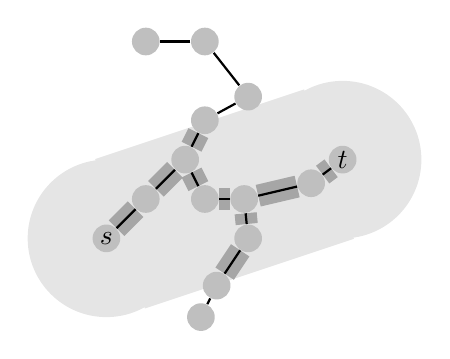
\begin{tikzpicture}  

    % Definition of the radii
    \def\firstradius{(0,0) circle (1cm)};
    \def\secondradius{(3, 1) circle (1cm)};

    \fill[filled] \firstradius;
    \fill[filled] \secondradius;
    
     % The real source and sink
    \foreach \pos/\name in {{(0,0)/s}, {(3, 1)/t}} {   
      \node[vertex] (\name) at \pos {$\name$};
    }
   
    \path[edgeBackground] (s) -- (t);

    % the extra nodes
    \foreach \pos/\name in \network
      \node[vertex] (\name) at \pos {};

    % The connections between them
    \foreach \source/\sink in {s/c, c/d, d/h, h/i, i/m, m/t, i/-, -/l, d/g}
      \path[real edge] (\source) -- (\sink);

    % The nodes they can reach
    \foreach \source/\sink in \connect
      \path[edge] (\source) -- (\sink);

\end{tikzpicture}}
% Remove empty line
\subfloat[Circle]{\label{fig:rdr2}
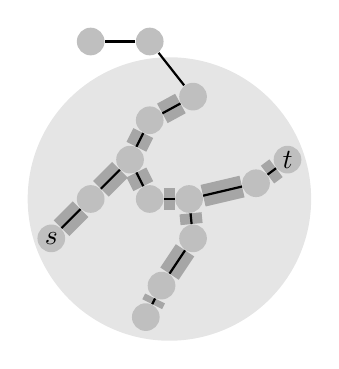
\begin{tikzpicture}  

    % Definition of the radii
    \def\radius{(1.5,0.5) circle (1.8)};
    \fill[filled] \radius;

     % The real source and sink
    \foreach \pos/\name in {{(0,0)/s}, {(3, 1)/t}} {   
      \node[vertex] (\name) at \pos {$\name$};
    }
   
    % the extra nodes
    \foreach \pos/\name in \network   
      \node[vertex] (\name) at \pos {};

    % The connections between them
   \foreach \source/\sink in {s/c, c/d, d/h, h/i, i/m, m/t, i/-, -/l, d/g, g/j, l/k}
      \path[real edge] (\source) -- (\sink);
 
    % The nodes they can reach
    \foreach \source/\sink in \connect
      \path[edge] (\source) -- (\sink);
\end{tikzpicture}}
% Remove empty line
\subfloat[Rectangle]{\label{fig:rdr3}
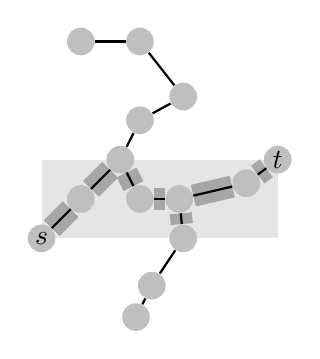
\begin{tikzpicture}  

    % Definition of the radii
    \def\rectangle{(0,0) rectangle (3,1)};
    \fill[filled] \rectangle;
 
     
    % The real source and sink
    \foreach \pos/\name in {{(0,0)/s}, {(3, 1)/t}}  
      \node[vertex] (\name) at \pos {$\name$};
   
    % the extra nodes
    \foreach \pos/\name in \network   
      \node[vertex] (\name) at \pos {};  

    % The connections between them
   \foreach \source/\sink in {s/c, c/d, d/h, h/i, i/-, i/m, m/t}
      \path[real edge] (\source) -- (\sink);
   
    % The nodes they can reach
    \foreach \source/\sink in \connect
      \path[edge] (\source) -- (\sink);
\end{tikzpicture}}
